%%%%%%%%%%%%%%%%%%%%%%%%%%%%%%%%%%%%%%%%
% Uppsala University Assignment Title Page 
% LaTeX Template
% Version 1.0 (27/12/12)
%
% This template has been downloaded from:
% http://www.LaTeXTemplates.com
%
% Original author:
% WikiBooks (http://en.wikibooks.org/wiki/LaTeX/Title_Creation)
% Modified by Elsa Slattegard to fit Uppsala university
% License:
% CC BY-NC-SA 3.0 (http://creativecommons.org/licenses/by-nc-sa/3.0/)

%\title{Title page with logo}
%----------------------------------------------------------------------------------------
%	PACKAGES AND OTHER DOCUMENT CONFIGURATIONS
%----------------------------------------------------------------------------------------

\documentclass[12pt]{article}
\usepackage{longtable}
\usepackage[english]{babel}
\usepackage[utf8x]{inputenc}
\usepackage{amsmath}
\usepackage{graphicx}
\usepackage{float}
\usepackage{multirow} % needed for tables
\setlength {\marginparwidth}{2cm}
\usepackage[colorinlistoftodos]{todonotes}
\usepackage{xcolor}
\usepackage{caption}
\usepackage{subcaption}
\usepackage{algorithm}
\usepackage{algpseudocode}
\usepackage{float}
\usepackage{biblatex}
\usepackage{amsthm}
\usepackage{algorithm}
\usepackage{algpseudocode}
\usepackage{amssymb}
\usepackage{csquotes}

\graphicspath{{../pdf/}{./MMPics/}}

\addbibresource{references.bib}

\newtheoremstyle{break}
  {\topsep}{\topsep}%
  {\itshape}{}%
  {\bfseries}{}%
  {\newline}{}%
\theoremstyle{break}
\newtheorem{definition}{Definition}[section]
\newtheorem{theorem}{Theorem}[section]
\newtheorem{corollary}{Corollary}[section]

\newcommand{\indep}{\perp \!\!\! \perp}

\newcommand\at[2]{\left.#1\right|_{#2}}

\begin{document}

\begin{titlepage}

\newcommand{\HRule}{\rule{\linewidth}{0.5mm}} % Defines a new command for the horizontal lines, change thickness here

\center % Center everything on the page
 
%----------------------------------------------------------------------------------------
%	HEADING SECTIONS
%----------------------------------------------------------------------------------------

\textsc{\LARGE Uppsala University}\\[1.5cm] % Name of your university/college

\includegraphics[scale=.1]{Uppsala_University_seal_svg.png}\\[1cm] % Include a department/university logo - this will require the graphicx package
\textsc{\Large Bachelor's Thesis}\\[0.5cm] % Major heading such as course name
% \textsc{\large 1TD070}\\[0.5cm] % Minor heading such as course title

%----------------------------------------------------------------------------------------
%	TITLE SECTION
%----------------------------------------------------------------------------------------

\HRule \\[0.4cm]
{ \huge \bfseries Martingale Matching}\\[0.4cm] % Title of your document
\HRule \\[1.5cm]
 
%----------------------------------------------------------------------------------------
%	AUTHOR SECTION
%----------------------------------------------------------------------------------------

\begin{minipage}{0.4\textwidth}
\begin{flushleft} \large
\emph{Authors:}\\
Anton \textsc{von Nandelstadh}\\% Your name
\end{flushleft}

\end{minipage}\\[2cm]

% If you don't want a supervisor, uncomment the two lines below and remove the section above
% \Large \emph{Author:}\\
% Benny \textsc{Avelin}\\[3cm] % Your name

%----------------------------------------------------------------------------------------
%	DATE SECTION
%----------------------------------------------------------------------------------------

{\large \today}\\[2cm] % Date, change the \today to a set date if you want to be precise

\vfill % Fill the rest of the page with whitespace

\end{titlepage}

\tableofcontents

\newpage

\section{Introduction}
This thesis aims to develop a novel method for learning the stochastic differential equation of a diffusion-based generative model, which we call martingale matching. We present this as an alternative to the predominant frameworks of score matching \cite{song2021} and flow matching \cite{lipman2023}.

The first diffusion models were discrete-time Gaussian processes \cite{sohldickstein2015, ho2020}. These were later reformulated as stochastic differential equations (SDEs) \cite{song2021}. In a diffusion model, the probability path interpolating between a simple distribution and the data distribution is created through a forward noising process modeled by an SDE. Inspired by the reversal of the forward noising process \cite{anderson1982}, these SDEs are chosen such that they have marginal probabilities which can parametrise the generator of the diffusion process using the score function, hence the name score matching \cite{song2020, lipman2024}. Our discussions regarding the framework of flow/score matching mostly follow the conventions used by \cite{lipman2024, holderrieth2026}. Specifically, we consider the SDE we want to learn as moving forward in time, unlike the theory of time-reversal used in the older score matching literature, such as \cite{song2021}.

Our novel approach is to learn the generator of the diffusion process directly, instead of using the score to do this implicitly. We do this by enforcing a known martingale from the basic theory of SDEs. We then use deviations from the martingale to construct a new loss function, based on which we train and learn the drift and diffusion functions. We present our results applying this new methodology to various toy datasets, and discuss the possibility of using it to train on high-dimensional data. In order to do this, we first develop some of the theory of stochastic differential equations, and the general theory of diffusion-based generative models.

\section{Background}
\subsection{SDE Preliminaries}
%Math part goes first
In order to understand denoising diffusion models, we first need to go through some preliminaries regarding stochastic processes and stochastic differential equations. In what follows, we assume basic knowledge of measure theory and measure-theoretic probability theory. We begin by expanding our regular probability space, defined by a triple, into a filtered probability space, defined by a quadruple.

\begin{definition}[Filtration]
	Let $(\Omega, \mathcal{F}, P)$ be a probability space and let $T$ be an ordered index set. For each $t \in T$, let $\mathcal{F}_t$ be a sub-$\sigma$-algebra of $\mathcal{F}$. Then $\{\mathcal{F}_t\}_{t \in T}$ is a filtration if $\mathcal{F}_k \subset \mathcal{F}_l$ for each $k \leq l$. Then $(\Omega, \mathcal{F}, \{\mathcal{F}_t\}, P)$ is called a filtered probability space.
\end{definition}

We are now ready for one of the central definitions of modern probability theory, that of a martingale.

\begin{definition}[Martingale]
	A stochastic process $X:T \times \Omega \to \mathbb{R}$ on a probability space $(\Omega, \mathcal{F}, P)$ is a martingale w.r.t. the filtration $\{\mathcal{F}_t\}$ (of $(\Omega, \mathcal{F}, P)$) if
	\begin{enumerate}
		\item
		X is adapted to the filtration. That is, $X_t$ is $\mathcal{F}_t$ measurable for each $t \in T$.
		\item
			For each $t$, $\mathbb{E}[|X_t|] < \infty$
		\item
			For all $s$ and $t$ with $s < t$, $\mathbb{E}[X_t|\mathcal{F}_s] = X_s.$
	\end{enumerate}
\end{definition}

A very important example of a martingale is that of Brownian motion.
	\begin{definition}[Brownian motion]
		The standard d-dimensional Brownian motion is a stochastic process $\{B_t\}$, $t \in [0, T]$, such that
		\begin{itemize}
			\item $B_0 = 0$
			\item for all $k$, and all $0 = t_0 < t_1 < \ldots < t_k = T$, the random variables \[B_{t_k} - B_{t_{k-1}} \sim N(0, (t_k - t_{k-1})I)\] are independent, where $I$ is the d-dimensional identity matrix.
			\item $B_t$ is almost surely continuous in $t$
		\end{itemize}
	\end{definition}

%We used to have the construction of the Itô integral here, so this should be revised so that the section makes sense without the construction.

	We now present the Itô integral, which is essential for our definition of stochastic differential equations. For the definition to be well-defined, we need to restrict the class of functions $\nu$ to which the definition applies. 

\begin{definition}
	Let $\nu = \nu(S, T)$ be the class of functions
	\begin{equation*}
		f(t, \omega):[0,\infty) \times \Omega \to \mathbb{R}
	\end{equation*}
	such that
	\begin{enumerate}
		\item
			$(t, \omega) \to f(t, \omega)$ is $\mathcal{B} \times \mathcal{F}$ measurable, where $\mathcal{B}$ denotes the Borel $\sigma$-algebra on $[0, \infty).$
		\item
			$f(t, \cdot)$ is $\mathcal{F}_t$ measurable for every $t$.
		\item 
			$\mathbb{E}[\int_S^T f(t, \omega)^2 dt] < \infty$.
	\end{enumerate}
	where $[S, T]$ is a time interval.
\end{definition}

Similarly to how the Lebesgue integral is constructed from simple functions, one can define a class of elementary functions, and then the integral of $f \in \nu$ can be defined as an $L^2$ limit of these elementary functions. 
\begin{definition}[Elementary function]
	A function $\phi \in \nu$ is called elementary if it has the form
	\begin{equation}
		\phi(t, \omega) = \sum_j e_j(\omega) \chi_{[t_j, t_{j+1})}(t).
	\end{equation}
	where the sum is taken over some finite partition and each $e_j$ is $\mathcal{F}_{t_j}$ measurable.
\end{definition}

Now, again similarly to how we do Lebesgue integration, we begin by defining the integral of the elementary functions with respect to Brownian motion.

\begin{definition}[Integral of an elementary function]
	For elementary function $\phi(t, \omega)$, the integral is defined according to
	\begin{equation}
		\int_S^T \phi(t, \omega) dB_t(\omega) = \sum_{j \geq 0} e_j(\omega)[B_{t_j + 1} - B_{t_j}](\omega).
	\end{equation}
\end{definition}

One can then show that for $f \in \nu$, one can choose elementary functions $\phi_n \in \nu$ converging to $f$ in $L^2$ norm. For a detailed construction of the Itô integral, see \cite{oksendal2013} or \cite{karatzas1998}. We get the definition below.

\begin{definition}[Itô integral]
	Let $f \in \nu(S,T)$. Then the Itô integral of $f$ (from $S$ to $T$) is defined by
	\begin{equation}
		\int_S^T f(t, \omega)dB_t(\omega) = \lim_{n \to \infty} \int_S^T \phi_n(t, \omega)dB_t(\omega)
	\end{equation}
	where $\{\phi_n\}$ is a sequence of elementary functions such that
	\begin{equation}
		\mathbb{E}\left[\int_S^T(f(t, \omega) - \phi_n(t, \omega))^2dt\right] \to 0 \quad \text{as } n \to \infty
	\end{equation}
\end{definition}

Note that by the construction \cite{oksendal2013}, the Itô integral of $f \in \nu$ is independent of which sequence of elementary functions we choose. The definition of the Itô integral can moreover be naturally extended to integration w.r.t. d-dimensional Brownian motion, see e.g. \cite{oksendal2013} or \cite{karatzas1998}. An important corollary of the construction of the Itô integral is the Itô isometry.

\begin{corollary}[Itô isometry]
	For $f \in \nu(S, T)$,
	\begin{equation}
		\mathbb{E}\left[\left( \int_S^T f(t, \omega) dB_t \right)^2\right] = \mathbb{E}\left[ \int_S^T f^2(t, \omega)dt \right]
	\end{equation}
\end{corollary}

Now we are ready to define stochastic differential equations. Stochastic differential equations are defined in terms of integral rather than derivatives. This is because the most common integrator, Brownian motion, is nowhere differentiable \cite{karatzas1998}. Hence its derivative is not defined.

\begin{definition}[Stochastic differential equation]
	A process $X_t$ satisfies the stochastic differential equation
	\begin{equation}
		dX_t = b(t, X_t)dt + \sigma(t, X_t)dB_t
	\end{equation}
	if it satisfies the integral equation
	\begin{equation}
		\label{eq:sde}
		X_t = X_0 + \int_0^t b(s, X_s) ds + \int_0^t \sigma (s, X_s) dB_s
	\end{equation}
	where $B_t$ is the standard d-dimensional Brownian motion.
\end{definition}

In order for an SDE to possess a unique strong solution, we must impose conditions on $\sigma$ and $b$. The proof of the following theorem is similar to the ODE case, where the proof of existence uses Picard iteration, and the proof of uniqueness uses the Itô isometry and the Lipschitz condition. The interested reader is referred to \cite{oksendal2013} or \cite{karatzas1998}.

\begin{theorem}[Existence and uniqueness of SDEs]
	\label{thm:existence}
	Let $T>0$ and $b:[0,T] \times \mathbb{R}^d \to \mathbb{R}^d, \sigma:[0, T] \times \mathbb{R}^d \to \mathbb{R}^{d \times k}$ be measurable functions satisfying
	\begin{equation}
		|b(t, x)| + |\sigma(t, x)| \leq C(1 + |x|) \quad x\in\mathbb{R}^d, t\in [0,T]
	\end{equation}
	for some constant $C$, $|\sigma|^2 = \sum|\sigma_{ij}|^2$, and such that
	\begin{equation}
		|b(t, x) - b(t,y)| + |\sigma(t,x)-\sigma(t,y)| \leq D|x-y| \quad x,y\in \mathbb{R}^d, t\in[0,T]
		\label{eq:lip}
	\end{equation}
	for some constant D. Let Z be a random variable which is independent of the $\sigma$-algebra generated by the Brownian motion, and such that
	\begin{equation}
		\mathbb{E}[|Z|^2] < \infty.
	\end{equation}
	Then the stochastic differential equation 
	\begin{equation}
		dX_t = b(t, X_t)dt + \sigma(t, X_t)dB_t, \quad 0 \leq t \leq T, \quad X_0 = Z
	\end{equation}
	has unique continuous (in t) solution $X_t$ with the property that $X_t$ is adapted to the filtration $\mathcal{F}_t^Z$ generated by $Z$ and $B_s, s \leq t$ and
	\begin{equation}
		\mathbb{E}\left[ \int_0^T |X_t|^2 dt\right] < \infty.
	\end{equation}

\end{theorem}

Now we are ready to state the central definition for our application, namely that of the Itô diffusion.

\begin{definition}[Itô diffusion]
	An Itô diffusion is a stochastic process $X_t(\omega) = X(t,\omega):[0,\infty) \times \Omega \to \mathbb{R}^d$ satisfying a stochastic differential equation of the form
	\begin{equation*}
		dX_t = b(t, X_t)dt + \sigma(t, X_t)dB_t, \quad t \geq s; X_s = x
	\end{equation*}
	where $B_t$ is k-dimensional Brownian motion and $b:[0, \infty) \times \mathbb{R}^d \to \mathbb{R}^d$, $\sigma:[0, \infty) \times \mathbb{R}^d \to \mathbb{R}^{d \times k}$ satisfy Eq. \ref{eq:lip}. We call $b$ the drift coefficient and $\sigma$ the diffusion coefficient.
\end{definition}


Note that the assumptions of Thm. \ref{thm:existence} simplify in the case of diffusion, in particular, linear growth follows from the Lipschitz condition. A very powerful result about Itô processes which we shall make use of is Itô's lemma. This is the stochastic equivalent of the chain rule in deterministic calculus.

\begin{theorem}[Itô's lemma]
	Let
	\begin{equation*}
		dX(t) = u dt + v dB(t)
	\end{equation*}
	be a d-dimensional Itô process. Let $f(t, x) = (f_1(t, x), \ldots, f_k(t, x))$ be a $C^2$ map from $[0,\infty) \times \mathbb{R}^d$ into $\mathbb{R}^k$. Specifically, let $f_k$ be continuously differentiable once in $t$ and twice in $x$. Then the process

	\begin{equation*}
		Y(t, \omega) = f(t, X(t))
	\end{equation*}

	is again an Itô process, whose $k$-th component $Y_k$, is given by

	\begin{equation*}
		dY_k = \frac{\partial f_k}{\partial t}(t,X)dt + \sum_{i}\frac{\partial f_k}{\partial x_i}(t, X)dX_i + \frac{1}{2}\sum_{i,j}\frac{\partial^2f_k}{\partial x_i \partial x_j} dX_i dX_j
	\end{equation*}

	where $dB_i dB_j = \delta_{i,j}dt$, $dB_idt = dtdB_i = dtdt = 0$. 
	
\end{theorem}

Note that the last line of the definition is a mnemonic. For a proof of Itô's lemma, see e.g. \cite{oksendal2013}. Another useful tool for us is the generator of the Itô diffusion, which encodes a lot of useful information about the diffusion process. Our algorithm learns the generator rather than learning the process directly.

\begin{definition}[Generator]
	Let $\{X_t\}$ be an Itô diffusion in $\mathbb{R}^d$. The generator $\mathcal{L}_t$ of $X_t$ at time $t$ is defined by
	\begin{equation*}
		\mathcal{L}_tf(x) = \lim_{h \downarrow 0}\frac{\mathbb{E}[f(X_{t+h})|X_t = x] - f(x)}{h}; \quad x \in \mathbb{R}^d
	\end{equation*}
	for the set $D(\mathcal{L}_t)$ of functions $f:\mathbb{R}^d \to \mathbb{R}$ where the limit exists uniformly.
\end{definition}

The generator exists for a wider class of processes than just Itô diffusion. However, in the case of diffusion, we can relate the generator to the drift and diffusion coefficients in the following way.

\begin{theorem}[Generator of diffusion]
	\label{thm:diffgen}
The generator of the diffusion process is given by

\begin{equation*}
	\mathcal{L}_t f = b_t \cdot \nabla f + \frac{1}{2} \mathrm{tr}(\sigma_t\sigma_t^T \nabla^2 f)	
\end{equation*}

which in the case where $\sigma$ is a scalar constant simplifies to 

\begin{equation*}
	\mathcal{L}_t f = b_t \cdot \nabla f + \frac{1}{2} \sigma^2 \Delta f	
\end{equation*}

Here $f$ is any $C^2_0$ function.
\end{theorem}

We refer the interested reader to \cite{karatzas1998} for the proof. Next, we relate the generator to a useful martingale. We call this Dynkin's formula, although there are stronger versions of it with the same name \cite{oksendal2013}.

\begin{theorem}[Dynkin]
Let $X_t$ be a diffusion process. Then $M_t^f$ is a martingale where

\begin{equation}
	\label{eq:mart}
	M_t^f = f(X_t) - f(X_0) - \int_0^t \mathcal{L}_s f(X_s) ds 
\end{equation}

so that $\mathbb{E}[M_t^f] = 0$. Here $f \in C^2_0$ is an arbitrary test function. $\mathcal{L}_t$ is the generator of the diffusion process.
\label{thm:mart}
\end{theorem}

\begin{proof}
	The Itô formula gives
	\begin{equation*}
		df(X_t) = \left(\sum_i b_i \frac{\partial f}{\partial x_i} + \frac{1}{2}\sum_{i,j}(\sigma \sigma^{T})_{i,j} \frac{\partial f}{\partial x_i \partial x_j} \right)dt + dM_t
	\end{equation*}

	where $M_t$ is some martingale term. We can rewrite this as 

	\begin{equation*}
		M_t = f(X_t) - f(x) - \int_0^t \mathcal{L}_sf(X_s)ds.
	\end{equation*}
\end{proof}

% \begin{proof}
% 	The Itô formula gives
% 	\begin{equation*}
% 		df(X_t) = \sum_i b_i \frac{\partial f}{\partial x_i} + \frac{1}{2}\sum_{i,j}(\sigma \sigma^{T})_{i,j} \frac{\partial f}{\partial x_i \partial x_j}dt + dM_t
% 	\end{equation*}
%
% 	where $M_t$ is some martingale term. We rewrite this as 
%
% 	\begin{equation*}
% 		f(X_t) = f(x) + \int_0^t \mathcal{L}f(X_s)ds + M_t
% 	\end{equation*}
%
% 	and we now wish to show that $\mathcal{L}f$ is the generator. Taking expectations we have
%
% 	\begin{equation*}
% 		\mathbb{E}^x[f(X_t)] = f(x) + \int_0^t \mathbb{E}_x[\mathcal{L}f(X_s)]ds + \mathbb{E}[M_t]
% 	\end{equation*}
%
% 	so that 
%
% 	\begin{equation*}
% 		\mathbb{E}^x[f(X_t)] - f(x) = \int_0^t \mathbb{E}^x[(\mathcal{L}f)(X_s)]ds
% 	\end{equation*}
%
% 	which gives us that
%
% 	\begin{equation*}
% 		\frac{d}{dt}\at{\mathbb{E}^x[f(X_t)]}{t=0} = \mathcal{L}f(x)
% 	\end{equation*}
%
% 	and so it is clear that $\|\frac{d}{dt}\mathbb{E}^x[f(X_t)] - \mathcal{L}f\|$ as $t \to 0$.
% \end{proof}

\subsection{Generative Models}
%CS part comes second
	A generative model allows us to interpolate between $p_{simple}$ and $p_{data}$. As the name suggests, we choose $p_{simple}$ to be some known distribution, so that we can easily generate new samples of $p_{data}$ by sampling $z \sim p_{simple}$ and applying the model. In this thesis, we define generative modelling as follows.

\begin{definition}[Generative modelling]
	Generative modelling is the process of training a model to transform a sample from a simple distribution $p_{simple}$ to a data distribution $p_{data}$. 
\end{definition}

In general, the distribution $p_{data}$ will be unknown to us, since otherwise there would not be much to learn. Instead, we assume access to a finite number of examples of $p_{data}$, sampled independently, which serves to represent the true distribution. We call this our dataset.
	
\begin{definition}[Dataset]
	A dataset is a finite number of i.i.d. samples $z_1,\ldots,z_N \sim p_{data}$.
\end{definition}

Our dataset might be a collection of images, such as MNIST, or a collection of videos. Our aim is then to train a model to generate more images of hand-written integers or videos. We shall also need the definition of a probability path.

\begin{definition}[Probability path]
	A probability path is a time-dependent probability $\{p_t\}_{0 \leq t \leq 1}$.
\end{definition}

An increasingly common class of generative models used are flow models. Here, one learns a vector field $b_t^{\theta}$, which parametrises the ODE that carries values from $p_{simple}$ to $p_{data}$ \cite{lipman2024}. Having learned $b_t^{\theta}$, one can then interpolate between the distributions simply using an ODE solver. 

\begin{definition}[Flow model]
	A flow model is given by:
	\begin{align*}
		\frac{d}{dt}X_t &= b_t^{\theta}(X_t) \\
		X_0 &\sim p_{simple}
	\end{align*} 
	where $b_t^{\theta}:[0,1] \times \mathbb{R}^d \to \mathbb{R}^d$ is a vector field parametrised by a neural network with parameters $\theta$.
\end{definition}

%Stuff here about how to train flow models i.e. flow matching
The way flow models are trained is called flow matching. Let $\mathcal{T} \in U([0,1])$ be a random time and $X_t \sim p_t$ our process. We construct a target vector field $u_t^{target}(x)$ and minimise the loss

\begin{equation*}
	L_{FM}(\theta) = \mathbb{E}[\|u_\mathcal{T}^{\theta}(X_\mathcal{T}) - u_\mathcal{T}^{target}(X_\mathcal{T})\|^2]
\end{equation*}

through stochastic gradient descent. One can construct the target as

\begin{equation*}
	u_t^{target}(x) = \int u_t^{target}(x|z)\frac{p_t(x|z)p_{data}(z)}{p_t(x)}dz
\end{equation*}

and then it holds that

\begin{equation*}
	X_0 \sim p_{simple}, \quad \frac{d}{dt}X_t = u_t^{target}(X_t) \implies X_t \sim p_t \quad (0 \leq t \leq 1)
\end{equation*}

\cite{lipman2024, holderrieth2025}. Unfortunately this integral is intractable, but one can show that the conditional flow matching loss, where $Z \sim p_{data}$

\begin{equation*}
	L_{CFM}(\theta) = \mathbb{E}[\| u_\mathcal{T}^{\theta}(X_\mathcal{T}) - u_\mathcal{T}^{target}(X_\mathcal{T}|Z)\|^2]
\end{equation*}

is the same as $L_{FM}(\theta)$, up to a constant, and so minimising one with gradient descent is equivalent to minimising the other \cite{lipman2024}, since their gradients coincide. 

Flow models were preceded by (denoising) diffusion models, which, in addition to the vector field, also have a stochastic component. The aim of classic score matching, is to learn the score, from which the parametrised drift $b_t^{\theta}$ can be derived. The diffusion coefficient $\sigma$ is chosen by us. Having learned the parametrised drift, we can generate new samples of our data distribution $p_{data}$, using one of many numerical SDE solvers. 

\begin{definition}[Diffusion model]
	A diffusion model is given by:
	\begin{align*}
		dX_t &= b_t^{\theta}(X_t)dt + \sigma_t d B_t \\
		X_0 &\sim p_{simple}
	\end{align*}
	where $b_t^{\theta}:[0,1] \times \mathbb{R}^d \to \mathbb{R}^d$ is the parametrised drift, $\sigma_t:[0,1] \to \mathbb{R}$ is our diffusion coefficient, and $p_{simple}$ is our initial data distribution.
\end{definition}

%Stuff here about the classical way to train diffusion models, i.e. score matching
The most common way to train diffusion models is through score matching \cite{song2021}. The presentation of score matching given here follows \cite{holderrieth2025, lipman2024} and is different, but equivalent to, the presentation given by \cite{song2021}. They prove the following theorem

\begin{theorem}
	Define the conditional and marginal vector fields $u_t^{target}(x|z)$ and $u_t^{target}(x)$ as above. Then, for diffusion coefficient $\sigma \geq 0$, we may construct an SDE which follows the same probability path, i.e.
	\begin{gather}
		X_0 \sim p_{simple}, \quad dX_t = \left( u_t^{target}(X_t) + \frac{\sigma^2}{2} \nabla \log p_t(X_t) \right) dt + \sigma dB_t \\
		\implies X_t \sim p_t \quad (0 \leq t \leq 1)
	\end{gather}

	In particular, $X_1 \sim p_{data}$, and this holds if we replace the marginal probability path and vector field with their conditional versions.
\end{theorem}

Now $\nabla \log p_t(x)$ is called the score, and we can write it as

\begin{equation*}
	\nabla \log p_t(x) = \int \nabla log p_t (x|z) \frac{p_t(x|z)p_{data}(z)}{p_t(x)}dz.
\end{equation*}

Similarly to flow matching, we approximate the score by a neural net $s_t^{\theta}$ and we can derive the losses

\begin{equation*}
	L_{SM} = \mathbb{E}[\|s_\mathcal{T}^{\theta}(X_\mathcal{T}) - \nabla \log p_\mathcal{T}(X_\mathcal{T})\|^2]
\end{equation*}

and

\begin{equation*}
	L_{CSM} = \mathbb{E}[\|s_\mathcal{T}^{\theta}(X_\mathcal{T}) - \nabla \log p_\mathcal{T}(X_\mathcal{T}|Z)\|^2].
\end{equation*}

Once again, $L_{SM}$ is intractable, but one can show that its gradient coincides with $L_{CSM}$.

Additionally, for Gaussian probability paths we can recover the vector field from the score or vice versa. This is why the traditional denoising diffusion models can be trained by only learning the score, since they are constructed based on Gaussian conditional probability paths \cite{song2021}.

Our algorithm, martingale matching, also learns the diffusion model, but using a different methodology than score matching. Instead of learning the vector field or score directly, we learn the generator of the process by enforcing a known martingale.

\section{Algorithm}
\subsection{Training}
Instead of constructing a loss using the marginal vector field, as in flow matching, or using the score, as in score matching, the idea of martingale matching is to enforce the martingale given by Thm. \ref{thm:mart}, and thereby to learn the generator of the process. As we saw previously, knowledge of the generator combined with knowledge of the diffusion coefficient is enough to know the drift.

Now, we are able to construct a loss function and learn the generator by enforcing that $M_t^f$ be a martingale. Since we already know $f$ and $\sigma$, learning the generator means we also learn the drift term $b_t^{\theta}$, as desired.

In practice, what we use is that we should have $\mathbb{E}[M_t^f] = 0$, and use deviations from this as our loss function. Thus, enforcing zero-mean allows us to learn the drift. This is how we construct our loss function.

Let 
\begin{equation*}
	0 = t_0 < t_1 < \ldots < t_N = T
\end{equation*}
be a time discretization of $[0,T]$. Let $i$ be the index of the batch, and let $f \in \mathcal{F}$ be a function in our set of test functions $\mathcal{F}$. Then for each sample of $p_{simple}$ and each time step, we get residual

\begin{equation*}
	\tilde R_{t_k}^{f,i} = f(X_{t_{k+1}}^i) - f(X_{t_k}^i) - \int_{t_k}^{t_{k+1}}\mathcal{L}_s^\theta f(X_s^i)ds
\end{equation*}

We use quadrature $\int_{t_k}^{t_{k+1}}\mathcal{L}_s^\theta f(X_s) ds \approx \Delta t_k \mathcal{L}_t^\theta f(X_{t_k})$, with $\Delta t = t_{k+1} - t_k$ small, to discretise the residuals and enable us to compute them efficiently. This gives discrete residual 

\begin{equation*}
	\tilde R_{t_k}^{f,i} = f(X_{t_{k+1}}^i) - f(X_{t_k}^i) - \Delta t \mathcal{L}_t^\theta f(X_{t_k}^i)
\end{equation*}

Our loss function is then simply the mean squared of these residuals. Now the loss function Eq. \ref{naive_loss} arises naturally, since $\frac{1}{N}\sum_{i=1}^N \tilde R \approx \mathbb{E}[\tilde R]$ for large $N$, which we know should be $0$.

\begin{equation}
	\label{naive_loss}
	L_1 = \frac{1}{T|\mathcal{F}|} \sum_{k=1}^{T} \sum_{f \in \mathcal{F}} \left(\frac{1}{N}\sum_{i=1}^{N} \tilde R^{f, i}\right)^2.
\end{equation}


Although Eq. \ref{naive_loss} is the mathematically cleanest version of our loss function, we made improvements not so much motivated by the theory but by their numerical superiority and displayed empirical improvements. 

First, we used a Monte-Carlo approach, as in Eq. \ref{bad_loss}, which significantly speeds up training by each summand being conditioned on a different value $z$ of our dataset.

\begin{equation}
	\label{bad_loss}
	L_2 = \frac{1}{|\mathcal{F}|} \sum_{f \in \mathcal{F}} \left(\frac{1}{N}\sum_{i=1}^{N} \tilde R^{f, i}\right)^2.
\end{equation}

Second, we changed our loss function so that instead of being genuinely pathwise, it becomes pathwise in a weak sense. Explicitly, we used the residual

\begin{equation}
	R_{t_k}^{f,i} = f(Y_{t_{k+1}}^i) - f(X_{t_k}^i) - \Delta t \mathcal{L}_t^\theta f(X_s^i)
\end{equation}

where $Y_{t_{k+1}} \sim p_{t_{k+1}}(\cdot|z)$ and $X_{t_k} \sim p_{t_k}(\cdot|z)$. Note that this significantly weakens the residual, in the sense that it is now not a pathwise statement about a diffusion process $X_t$, but a statement about the random variables $Y_{t_{k+1}}$ and $X_{t_k}$. Nevertheless, it is numerically preferable, since we have that $Y_{t_{k+1}} \indep X_{t_k} \ | \ Z$, where $Z \sim p_{data}$. The residual $R_{t_k}^{f, i}$ gives the loss function

\begin{equation}
	\label{better_loss}
	L_3 = \frac{1}{|\mathcal{F}|} \sum_{f \in \mathcal{F}} \left(\frac{1}{N}\sum_{i=1}^{N} R^{f, i}\right)^2.
\end{equation}

Intuitively, minimising the loss function $L_3$ implies weak generator learning. We formalise this as follows.

\begin{theorem}[Weak moment matching]
	Let $\tilde X_t \sim p_t(\cdot|z)$ be a process. If for each $f \in \mathcal{F}$ we have that $\mathbb{E}[R^f_t] = 0$, $\mathbb{E}[\mathcal{L}_sf(\tilde X_s)] \in C([t,t+\Delta t])$ then 

\begin{equation}
	\mathbb{E}[\mathcal{L}_t f(\tilde X_t)] = \mathbb{E}[\mathcal{L}_t^\theta f(\tilde X_t)] \quad \text{as } \Delta t \to 0.
\end{equation}
\end{theorem}

\begin{proof}
	We have that

	\begin{equation}
		\mathbb{E}[R^f_t] = \mathbb{E}[f(Y_{t+\Delta t})] - \mathbb{E}[f(X_t)] - \Delta t \mathbb{E}[\mathcal{L}_t^\theta f(X_t)] = 0.
		\label{eq:ered}
	\end{equation}

	where $X_t \sim p_t(\cdot|z)$ and $Y_{t+\Delta t} \sim p_{t + \Delta t}(\cdot | z)$ are only defined at points $t$ and $t + \Delta t$ respectively. Using that $X_t \sim \text{Law}(\tilde X_t)$ and $Y_{t+\Delta t} \sim \text{Law}(\tilde X_{t + \Delta t})$, we can rewrite (\ref{eq:ered}) as (\ref{eq:fract1})

	\begin{equation}
		\mathbb{E}[\mathcal{L}_t^\theta f(\tilde X_t)] = \frac{\mathbb{E}[f(\tilde X_{t+\Delta t})] - \mathbb{E}[f(\tilde X_t)]}{\Delta t}.
		\label{eq:fract1}
	\end{equation}

	Additionally, Dynkin gives

	\begin{equation}
		\frac{\mathbb{E}[f(\tilde X_{t+\Delta t})] - \mathbb{E}[f(\tilde X_t)]}{\Delta t} = \frac{1}{\Delta t} \int_t^{t+\Delta t}\mathbb{E}[\mathcal{L}_s f(\tilde X_s)]ds.
		\label{eq:fract2}
	\end{equation}

	Combining (\ref{eq:fract1}) and (\ref{eq:fract2}) we get

	\begin{equation}
		\mathbb{E}[\mathcal{L}_t^\theta f(\tilde X_t)] = \frac{1}{\Delta t} \int_t^{t+\Delta t}\mathbb{E}[\mathcal{L}_sf(\tilde X_s)]ds.
	\end{equation}

	Taking limits gives

	\begin{equation}
		\lim_{\Delta t \to 0} \mathbb{E}[\mathcal{L}_t^\theta f(\tilde X_t)] = \mathbb{E}[\mathcal{L}_t(\tilde X_t)].
	\end{equation}
\end{proof}

If we now write $\epsilon = \mathbb{E}[\mathcal{L}_tf(X_t) - \mathcal{L}_t^\theta f(X_t)]$ as our error, then heuristically 

\begin{equation}
	\min_\theta \left( \frac{1}{N} \sum_{i=1}^N R_\theta^{f, i}\right)^2 \approx {\Delta t}^2 \epsilon^2 \quad \text{as }\Delta t \to 0.
	\label{eq:order}
\end{equation}


The loss $L_3$ is directly justified by the weak martingale
condition. In practice, we use the stronger surrogate $L_{ME}$, obtained by
moving the square inside the empirical average. Since
\[
    \mathbb{E}\bigl[(R_\theta^f)^2\bigr]
    =
    \bigl(\mathbb{E}[R_\theta^f]\bigr)^2
    +
    \operatorname{Var}(R_\theta^f),
\]
this surrogate can be interpreted as augmenting the moment-matching objective
with a variance penalty on the residuals. Although this modification is not
implied by the martingale identity alone, and may in principle change the
population minimiser, we find empirically that it gives more stable and faster
training.

\begin{equation}
	\label{best_loss}
	L_{ME} = \frac{1}{|\mathcal{F}|N} \sum_{f \in \mathcal{F}} \sum_{i=1}^{N} (R^{f, i})^2.
\end{equation}

With our loss constructed, we can now create our martingale matching algorithm, which is similar in spirit to other algorithms for generative modelling, such as flow and score matching. The algorithm is given in Alg. \ref{alg:mm}. Note that we use constant scalar $\sigma$ for simplicity.

\begin{algorithm}
	\caption{Martingale Matching}\label{alg:mm}
	\begin{algorithmic}
		\Require Neural net $b_t^{\theta}$, diffusion coefficient $\sigma$, time-step $\Delta t$, dataset of samples $z \sim p_{data}$, conditional probability path $p_t(\cdot|z)$
		\For{each minibatch of data}
		\State Sample z from minibatch.
		\State Sample $t \sim U[0,1-\Delta t]$.
		\State Set $x_t \sim p_t(\cdot|z)$, $x_{t+\Delta t} \sim p_{t + \Delta t}(\cdot|z)$.
		\State Compute loss $L_{ME}$.
		\State Update the model parameter $\theta$ via gradient descent on $L_{ME}$.
		\EndFor	
	\end{algorithmic}
\end{algorithm}


One of the main hyperparameters thus becomes our test function, and the choice of test functions is the major design decision in any implementation of this algorithm. We want to choose a subset of functions that are sufficiently rich to learn the drift, but computationally inexpensive. Because this choice is rather arbitrary, many modern generative methods try to avoid it altogether \cite{holderrieth2025}. 
One set of test functions is that of random Fourier features. These have the advantage of being computationally fast, particularly for higher dimensional data, as the number of functions required does not necessarily depend on the dimension of the data.

\begin{definition}[Random Fourier features]
	A random Fourier feature is a function of the type 
	\begin{equation*}
		f_{\omega_1}(x) = cos(w^\intercal x) \quad f_{\omega_2}(x) = sin(w^\intercal x)
	\end{equation*}
	where $x \in \mathbb{R}^d$ and $\omega \sim N(0, I_d)$.
\end{definition}

Another intuitive test function to try is that of polynomials. We found empirically that these work better than the Fourier features, but they have the disadvantage that they are computationally heavier, since the number of test functions of degree $k$ is ${k + d \choose k}$, where $d$ is the dimension of our data. This means that we are restricted to both low-degree polynomials and low-dimensional data.

\begin{definition}[Polynomial test functions]
	Suppose our dataset has dimension $d$. Then we call the set of monomials in $d$ variables of degree up to $k$ the set of polynomial test functions.
\end{definition}

Another set of test functions is Hermite polynomials. We did not find much empirical improvement over regular polynomial test functions, and hence our analysis focused on comparing random Fourier features with polynomials.

\begin{definition}[Hermite polynomial test functions]
	\begin{equation*}
		He_n(x) = (-1)^n e^{\frac{x^2}{2}}\frac{d^n}{dx^n}e^{-\frac{x^2}{2}}
	\end{equation*}
\end{definition}


The polynomial test functions, in addition to performing quite well empirically, have the additional advantage of having quite a nice mathematical interpretation. Consider $X_t$, $Y_t$ modelled by Alg. \ref{alg:mm}, and the Markov operator defined by

\begin{equation}
	K_{t,\Delta t} f(x) = \mathbb{E}[f(Y_{t+\Delta t})|X_t = x].
\end{equation}

We can use the Markov operator to characterize the minimiser of $L_{ME}$, as in the following theorem.

\begin{theorem}
	Suppose $f \in C^2_0$. Then the minimiser of

	\begin{equation}
		\min_{F \in L^2(\Omega)}\mathbb{E}[(f(Y_{t+\Delta t}) - f(X_t) - \Delta t F)^2]
	\end{equation}

	is given by

	\begin{equation}
		F = \frac{K_{t,\Delta t} f(x) - f(x)}{\Delta t} \quad p_t-a.e.
	\end{equation}
\end{theorem}

\begin{proof}
	Note that we have that $X_t \sim p_t(\cdot|z)$, $Y_{t+\Delta t} \sim p_t(\cdot|z)$ and $X_t \indep Y_{t + \Delta t} \ | \ Z$, so that we can condition on $X_t = x$ to give us
	\begin{equation}
		\mathbb{E}[(f(Y_{t+\Delta t}) - f(x) - \Delta t F)^2 | X_t = x].
	\end{equation}

	This is a standard least-squares problem which is minimized when by

	\begin{align*}
		F &= \mathbb{E}[f(Y_{t+\Delta t}) - f(x)| X_t = x] \\ 
		  &= \mathbb{E}[f(Y_{t+\Delta t}) | X_t = x] - f(x).
	\end{align*}
\end{proof}

Note that although $F$ in general is not parametrisable by a fixed neural network, we learn an approximate $F$ using $\mathcal{L}_t^\theta f(x)$. 
Now we may look at what the generator becomes for various test functions, by simply plugging them into the formula Thm. \ref{thm:diffgen}. For coordinate test functions $f_j(x) = x_j$ we find that

\begin{equation}
	\mathcal{L}_t^\theta f_j = b_j^\theta
\end{equation}

so that we simply learn the drift. However, we found better empirical performance when including higher-order terms. Second degree polynomial terms $f(x) = x_i x_j$ give us

\begin{equation}
	\mathcal{L}_t (x_i x_j) = x_jb_i(x, t) +  x_i b_j(x,t) + a_{i,j}(x, t)
\end{equation}
where $a = \sigma \sigma^T$. In particular, for $a = \sigma^2 I$, which we use, we get

\begin{align*}
	\mathcal{L}_t(x_i^2) &= 2x_ib_i(x,t) + \sigma^2 \\
	\mathcal{L}_t(x_i x_j) &= x_j b_i(x,t) + x_i b_j(x, t).
\end{align*}

A key step in Alg. \ref{alg:mm} is that of sampling $p_t(.|z)$ to generate our values $x$. In order to do this we need to develop our concept of conditional probability paths. The most common probability path used in generative flow models is a Gaussian probability path.

\begin{definition}[Gaussian probability path]
	Let $\alpha_t = \alpha(t) \in C^1([0,1])$ and $\beta_t = \beta(t) \in C^1([0,1])$ be noise schedulers, that is, monotonic functions with $\alpha_0 = \beta_1 = 0$ and $\alpha_1 = \beta_0 = 1$. We then define the Gaussian conditional probability path to be

	\begin{equation*}
		p_t(\cdot|z) = N(\alpha_tz, \beta_t^2 I_d).
	\end{equation*}

	Then this probability path fulfills the boundary conditions
	\begin{equation*}
		p_0(\cdot|z) = N(\alpha_0z, \beta_0^2 I_d) = N(0, I_d)\quad and \quad p_1(\cdot|z) = N(\alpha_1 z, \beta_1^2 I_d) = \delta_z.
	\end{equation*}
\end{definition}

Score matching widely uses Gaussian probability paths. However, Gaussian probability paths have the inherent restrictions that they force $p_{simple}$ to also be Gaussian. Hence, if one wants to interpolate between arbitrary distributions, one must use some other probability path.

However, we found that, in practice, $p_{simple}$ is chosen for convenience provided that it is easy to sample from. Hence, Gaussian probability paths often suffice, which is why we relied on them.

\subsection{Generation}
Having learned our drift $b_t^{\theta}$, we want to use it to generate new samples in $p_{data}$ from our synthetic distribution $p_{simple}$. We can do this by simply solving the stochastic differential equation, and thus simulating its path. In our implementation we use the Euler-Maruyama solver, since it is very simple. Alg. \ref{alg:euler} gives the pseudocode.

\begin{algorithm}[H]
	\caption{Euler-Maruyama}\label{alg:euler}
	\begin{algorithmic}
		\Require Neural net $b_t^{\theta}$, number of steps n, diffusion coefficient $\sigma_t$
		\State Set $h = \frac{1}{n}$
		\State Set $t=0$
		\State Sample $X_0 \sim p_{simple}$
		\For{$i = 1, \ldots, n$}
		\State Sample $\epsilon \sim N(0, I)$
			\State $X_{t+h} = X_t + h b_t^{\theta} (X_t) + \sigma_t \sqrt{h} \epsilon$
			\State Update $t \leftarrow t + h$
		\EndFor
		\State \Return $X_1$
	\end{algorithmic}
\end{algorithm}

The Euler-Maruyama method is essentially just the Euler method for deterministic differential equations, but with some simulated noise. At each time-step, the Euler-Maruyama method takes a step in the direction predicted by our neural net $b_t^{\theta}$, while adding some noise to approximate the stochastic component. This is the main part of the algorithm, namely updating the time step:

\begin{equation*}
	X_{t+h} = X_t + h b_t^{\theta} (X_t) + \sigma_t \sqrt{h} \epsilon
\end{equation*}

The Euler-Maruyama method converges in the following sense.

\begin{definition}
	The time discrete approximation $Y^\delta$, with maximum step size $\delta$, converges strongly to the Itô process X with order $\gamma > 0$ at time $T$ if there exists constant $C>0$ and $\delta_0 > 0$ such that
	\begin{equation*}
		\epsilon(\delta) = \mathbb{E}\left[\left|X_t - Y^\delta (T)\right|\right] \leq C\delta^\gamma.
	\end{equation*}
\end{definition}

One can show that the Euler-Maruyama method converges strongly with order 0.5, under the conditions of Thm. \ref{thm:existence}. \cite{kloeden1999} For more about the Euler-Maruyama method and other methods for solving SDEs, we refer the interested reader to \cite{kloeden1999}. 
We can now generate new samples of our $p_{data}$ distribution, simply by sampling $p_{simple}$, and simulating the SDE using Euler-Maruyama to get from $X_0 \sim p_{simple}$ to $X_1 \sim p_{data}$.

\section{Results}
We implemented Alg. \ref{alg:mm} using two of the test functions we suggested. Since we did not see a significant difference between the regular and Hermite polynomial test functions, we present the results for regular polynomial test functions here. For our implementation, we parametrised the drift using an MLP neural network of size $4 \times 64$, $4$ layers each of width $64$. We used $\sigma = 0.5$, as well as $1000$ SDE time-steps and a batch size of $10000$ with $5000$ epochs of training. The hyperparameters were chosen through initial empirical experimentation, while keeping computation fairly fast (at most a few minutes) on an Apple M3 Pro CPU.

We began by learning a mixture of Gaussians. This is perhaps the most natural distribution for us to learn, since we are using Gaussian probability paths and we have the Gaussian noise component of the stochastic differential equation as well. For this distribution, we got very good results with all of our test functions, hence we only present the result of Fourier test functions. An example of the flow of samples and trajectories of the learned model, compared with the ground-truth Gaussian probability paths, is given in Fig. \ref{fig:gaussF}. The ground-truth probability paths are simply Gaussian probability paths interpolating between $p_{simple}$ which is Gaussian, and $p_{data}$.

\begin{figure}[H]
  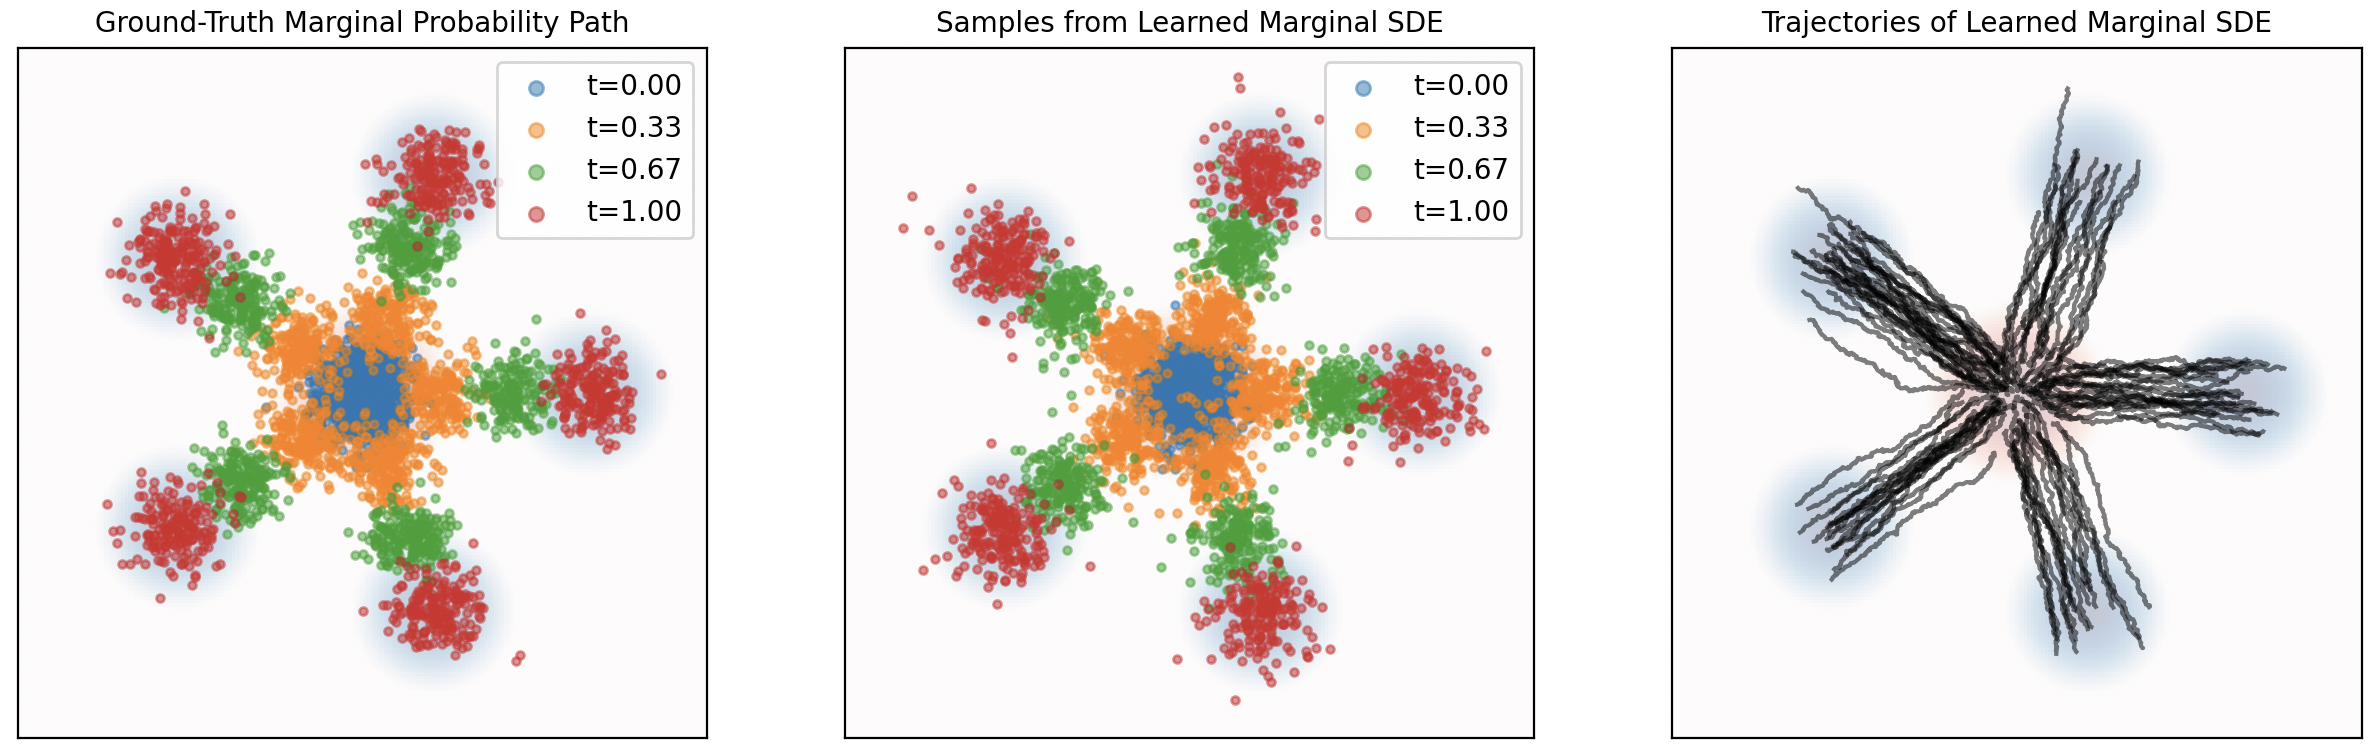
\includegraphics[width=\linewidth]{gauss.png}
  \caption{Illustration of learning Gaussian mixtures. (Left) Samples from the ground-truth probability path at different times; (Middle) Samples from the learned marginal SDE; (Right) Trajectories of the learned marginal SDE.}
  \label{fig:gaussF}
\end{figure}

To distinguish between the quality of different test functions, we had to train on more difficult data distributions. However, we only used $2d$ distributions. This is largely because they are easy to visualize. Moreover, we encountered some problems with higher-dimensional data, which are discussed below. Fig. \ref{fig:moonF} shows the flow of data learned using Fourier test functions, compared to the ground-truth probability paths. Fig. \ref{fig:checkF} shows the results for learning a checkerboard data distribution and Fig. \ref{fig:circlesF} the results for a circles distribution.

\begin{figure}[H]
  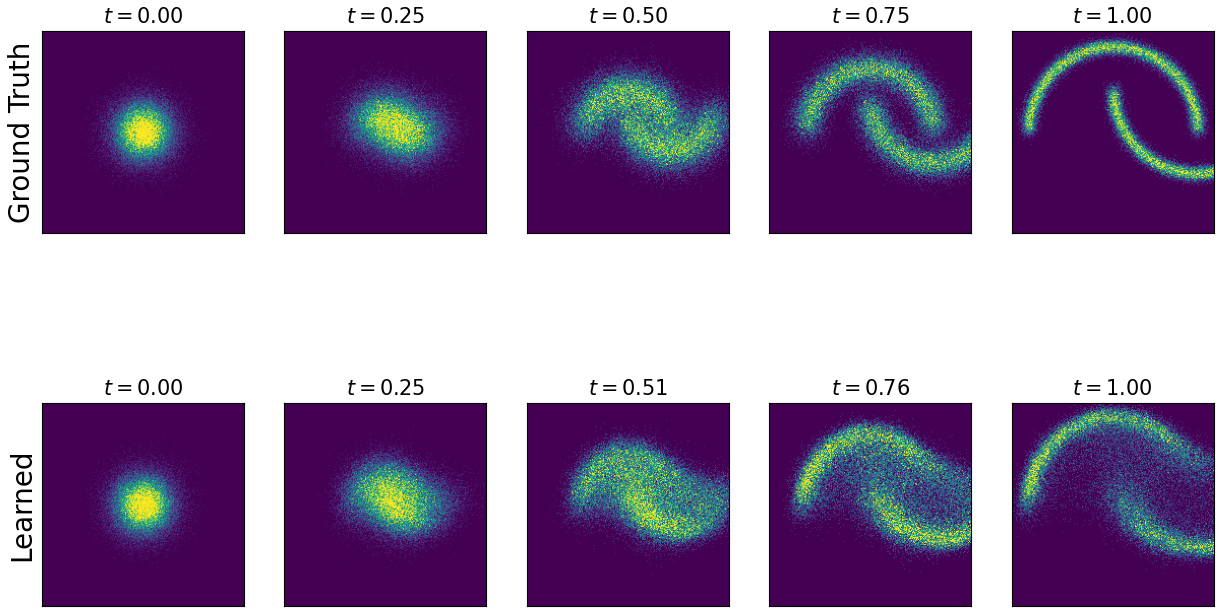
\includegraphics[width=\linewidth]{moons_fourier.png}
  \caption{Illustration of learning the two moons dataset using Fourier test functions. (Top) The ground-truth Gaussian probability path, sampled at various times; (Bottom) The learned probability paths, sampled at the same times.}
  \label{fig:moonF}
\end{figure}

\begin{figure}[H]
  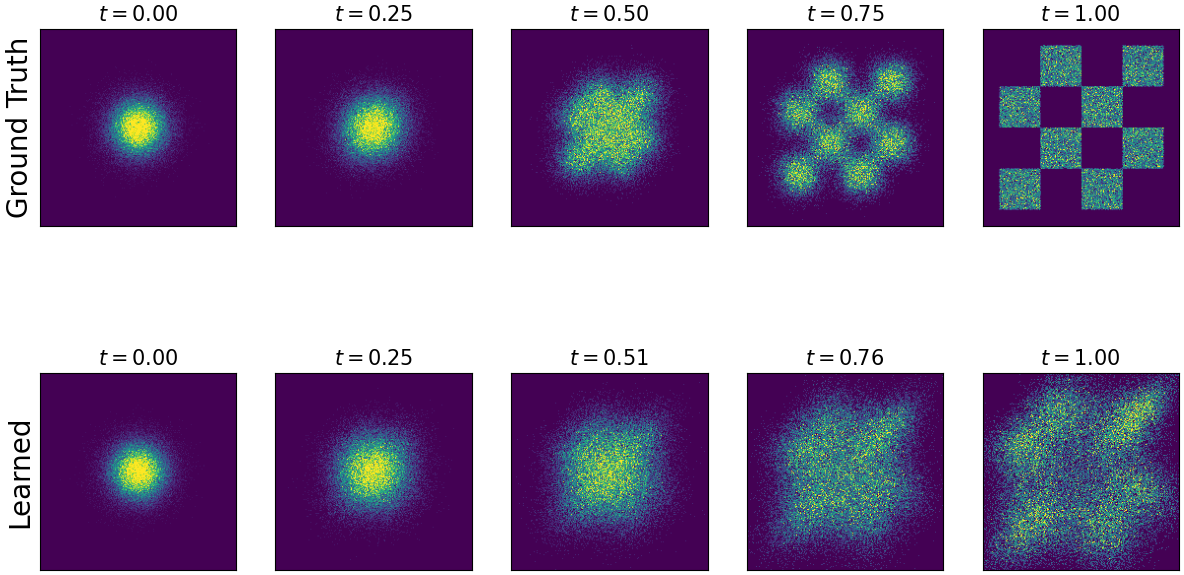
\includegraphics[width=\linewidth]{checkerboard_fourier.png}
  \caption{Illustration of learning the checkerboard dataset using Fourier test functions. (Top) The ground-truth Gaussian probability path, sampled at various times; (Bottom) The learned probability paths, sampled at the same times.}
  \label{fig:checkF}
\end{figure}

\begin{figure}[H]
  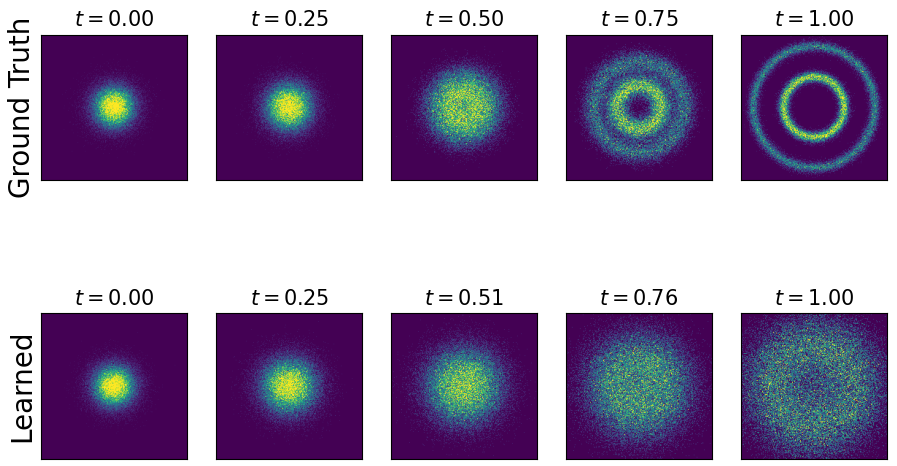
\includegraphics[width=\linewidth]{circles_fourier.png}
  \caption{Illustration of learning the circles dataset using Fourier test functions. (Top) The ground-truth Gaussian probability path, sampled at various times; (Bottom) The learned probability paths, sampled at the same times.}
  \label{fig:circlesF}
\end{figure}

As seen in Fig. \ref{fig:moonF} and Fig. \ref{fig:checkF}, the Fourier functions seem to struggle with even slightly more complicated data than Gaussian mixtures. As soon as Fourier test functions are used to learn a drift which is clearly non-linear, the algorithm struggles. The Fourier test functions seem to especially struggle on the checkerboard, but here no stochastic process with non-zero diffusion at time $t=1$ will learn the distribution perfectly, since the stochastic component will always make the corners slightly fuzzy. However, the Fourier test functions seem to learn very little in Fig. \ref{fig:circlesF}, which shows that the problem does not lie with "sharp corners".

Hence, we then implemented polynomial test functions up to the second degree on the same data sets. Fig. \ref{fig:moonP} shows two moons and Fig. \ref{fig:checkP} shows the checkerboard, both learned using polynomial test functions. We find that the polynomial test functions do much better than the Fourier features. They are likely able to better learn higher-order terms of the drift. The polynomial test functions learn the two moons dataset almost perfectly, and the checkerboard with much less fuzziness than the Fourier test functions. Moreover, Fig. \ref{fig:circlesP} shows that the polynomial test functions learn the circles dataset almost perfectly.


\begin{figure}[H]
  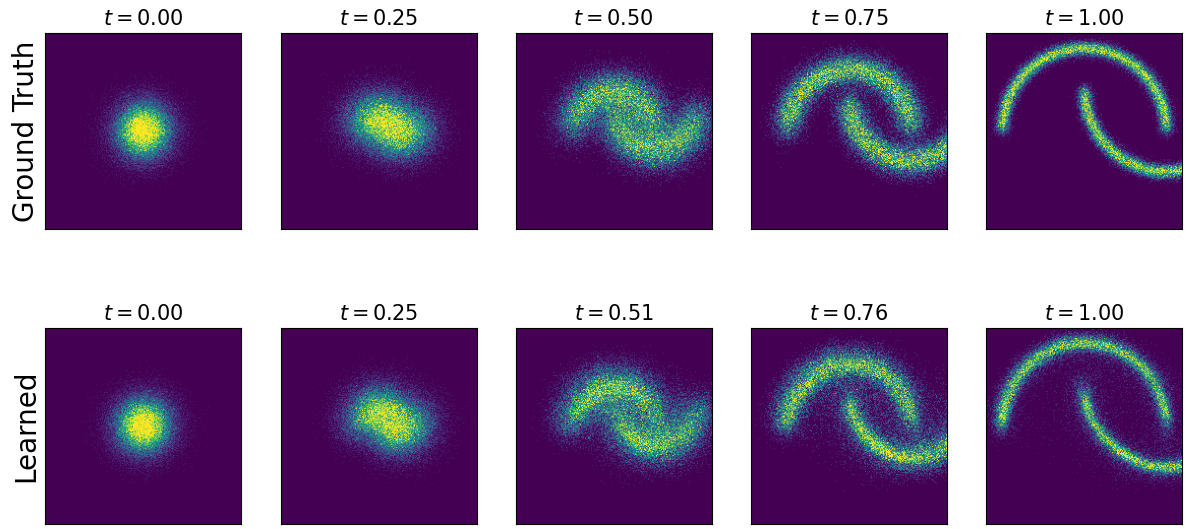
\includegraphics[width=\linewidth]{moons_poly.png}
  \caption{Illustration of learning the two moons dataset using polynomial test functions. (Top) The ground-truth Gaussian probability path, sampled at various times; (Bottom) The learned probability paths, sampled at the same times.}
  \label{fig:moonP}
\end{figure}


\begin{figure}[H]
  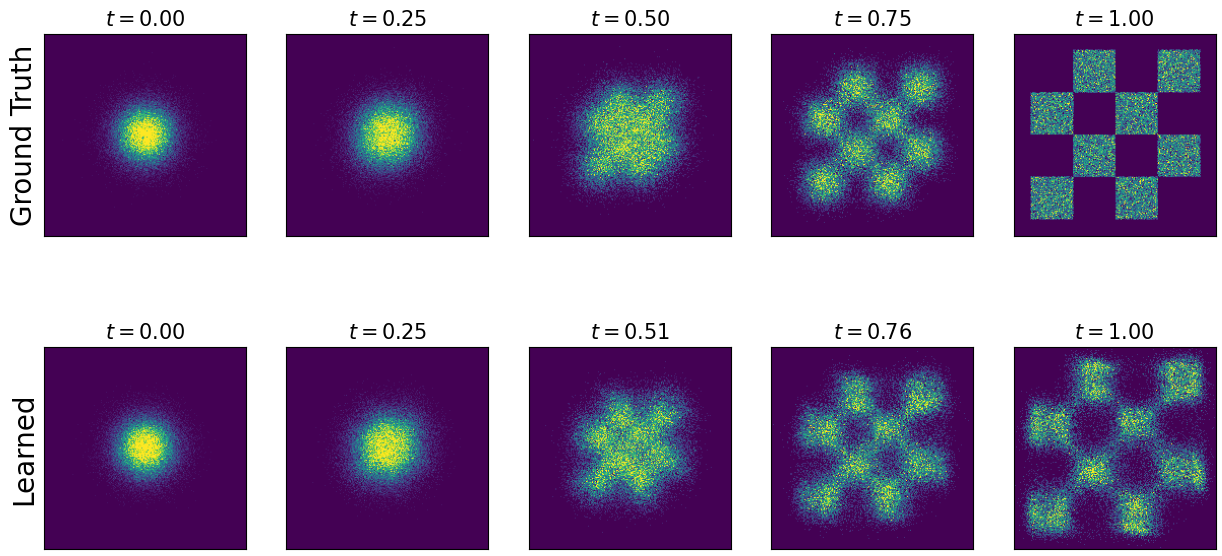
\includegraphics[width=\linewidth]{checkerboard_poly.png}
  \caption{Illustration of learning the checkerboard dataset using polynomial test functions. (Top) The ground-truth Gaussian probability path, sampled at various times; (Bottom) The learned probability paths, sampled at the same times.}
  \label{fig:checkP}
\end{figure}

\begin{figure}[H]
  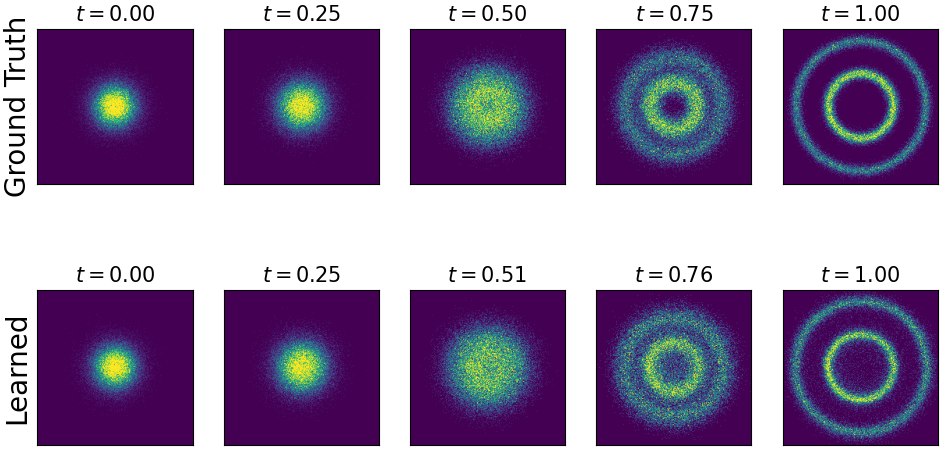
\includegraphics[width=\linewidth]{circles_poly.png}
  \caption{Illustration of learning the circles dataset using polynomial test functions. (Top) The ground-truth Gaussian probability path, sampled at various times; (Bottom) The learned probability paths, sampled at the same times.}
  \label{fig:circlesP}
\end{figure}

We also attempted to learn higher-dimensional data, such as the MNIST dataset of handwritten digits with $28 \times 28$ pixels, which has dimension $28 \times 28 = 784$. However, we encountered the problem that our Fourier test functions were not good enough, whereas the number of our second-degree polynomial test functions grow quadratically. This means that in the MNIST case, we have ${784 + 2 \choose 2} = 308505$ test functions. This significantly slows down our computation, and more importantly, requires too much memory to run on a regular computer.

\section{Conclusion}
The results we got applying martingale matching to toy data were very encouraging. Clearly we are able to learn something useful about our data simply by enforcing the martingale given in Eq. $\ref{eq:mart}$. The main architectural difficulty we encountered was finding test functions which give us good results while being computationally cheap.

Hence, there are a multitude of ways to extend this work, since the primary design choice for martingale matching is how we choose test functions. One option would be to look at different test functions than Fourier features or polynomials. Our choice of test functions was somewhat arbitrary, and there are surely alternatives that would perform
better. Another would be to try to mitigate the weaknesses of different test functions by combining them in various ways, to better represent the whole space of test functions. 

Perhaps the most promising extension would be to learn the test functions. If one were to parametrise them by their own neural nets, then one could simply train them while training the drift. This would remove some of the design choices that have to be made while implementing the martingale matching algorithm. More importantly, it would likely decrease the number of test functions needed and significantly improve the scalability to higher dimensions. This is because a dataset like MNIST, although it has $784$ pixels, in reality has many fewer true dimensions. Hence, many of the relationships captured by mixed-term polynomials likely do not contribute meaningfully to the learning process, and hence could be discarded. We hypothesize that the machine could do quite a good job at choosing the meaningful dimensions through learning.

\nocite{*}
\printbibliography

\end{document}

